\documentclass{scrartcl}
 
\usepackage[utf8]{inputenc}
\usepackage[T1]{fontenc}
\usepackage{lmodern}
\usepackage{listings}
\usepackage[english]{cleveref}
\usepackage[english]{babel}
\usepackage{graphicx}



\usepackage{float}




\newcommand{\code}[1]{{\fontfamily{cmtt}\small\selectfont#1}}
\newcommand{\codefs}[1]{{\fontfamily{cmtt}\scriptsize\selectfont#1}}


% multiline comments
\usepackage{verbatim} 

\usepackage{color}
\usepackage{listings}

%  basicstyle=\sffamily\small,


\lstdefinelanguage{Scala}{
	morekeywords={},
	morekeywords=[2]{
		public, private, protected,
		abstract,case,catch,class,def,
		do,else,extends,false,final,finally,
		for,if,implicit,import,match,mixin,
		new,null,object,override,package,
		private,protected,requires,return,sealed,
		super,this,throw,trait,true,try,
		type,val,var,while,with,yield,
		lazy,evt,observable,imperative,
                after,before},
	otherkeywords={=>,<-,<\%,<:,>:,\#,@},
	sensitive=true,
	morecomment=[l]{//},
	morecomment=[n]{/*}{*/},
	morestring=[b]",
	morestring=[b]',
	morestring=[b]"""
}
\lstloadlanguages{Scala}

\lstset{
  backgroundcolor=\color{white},%\fontfamily{cmtt}
  basicstyle=\fontfamily{cmtt}\scriptsize,
  basewidth=0.5em,
  showstringspaces=false,
  keywordstyle=\fontfamily{pcr}\color[rgb]{0,0,0}\bfseries,
  %commentstyle=\color[rgb]{0.133,0.545,0.133},
  %stringstyle=\color[rgb]{0.627,0.126,0.941},
  breaklines=false,
  frame=none
  breaklines=false,
  frame=none,
  numbers=left, numberstyle=\tiny, stepnumber=1, numbersep=5pt,
  %frameround=fttt,
  %frame=single,
  escapeinside={(*@}{@*)},
  %columns=fullflexible
}

\lstnewenvironment{codenv}{\lstset{language=Scala}}{}


\title{ReSwing -- A Reactive Interface for Scala Swing}
\author{}
\date{}
\begin{document}

\maketitle






\section{RESwing}

The RESwing library is an extension of the Scala Swing library, which
wraps around Java Swing. The Scala Swing library mirrors the Java
Swing class hierarchy and every component holds a reference to the
underlying Java Swing component. Building on Scala Swing, the RESwing
library adds another layer to this architecture. It provides its own
class hierarchy containing all reactively enabled
components. Figure~\ref{fig:overview} shows a small, representative
part of these class hierarchies.

\begin{figure}[htp]
  \centering
  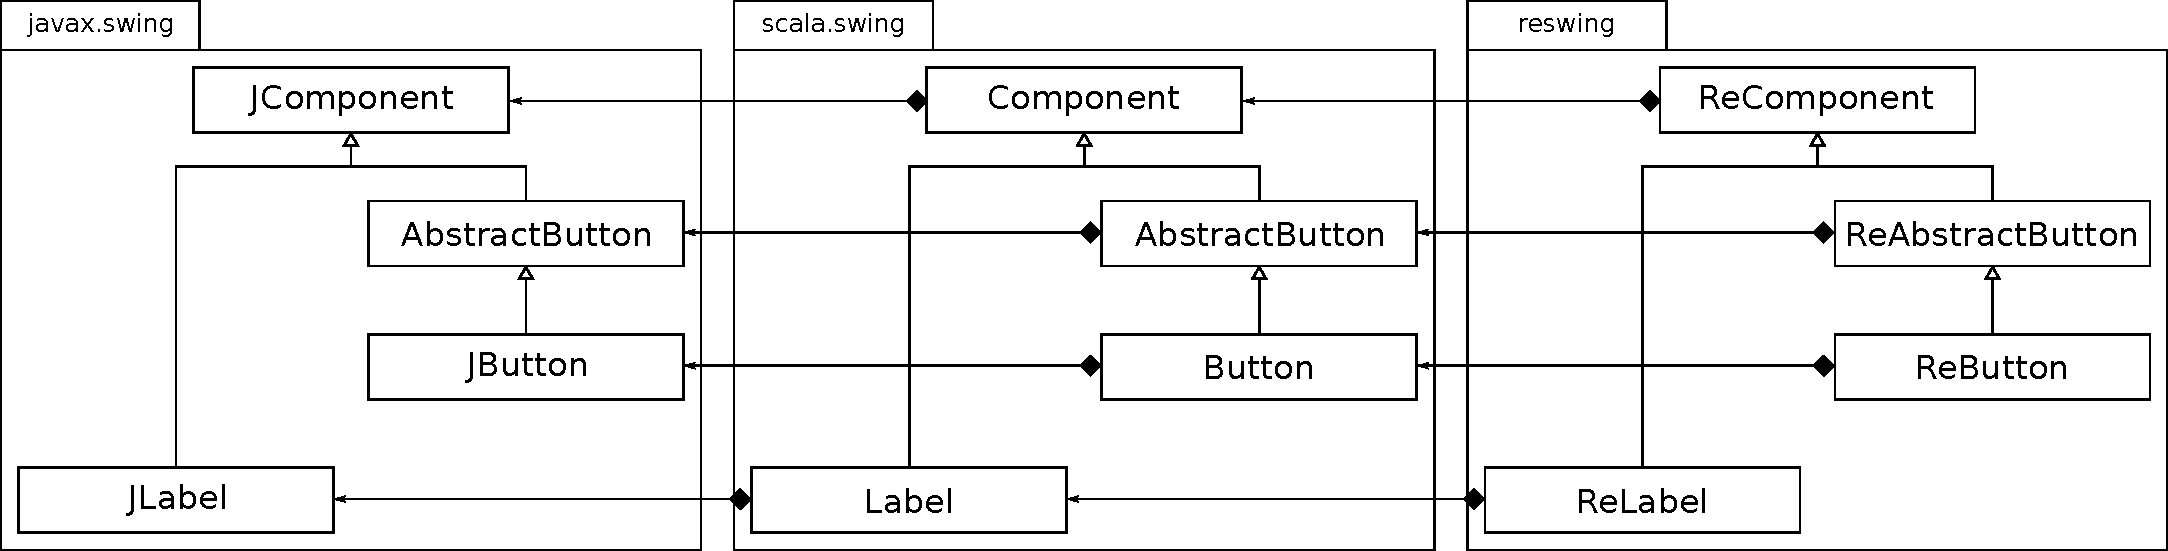
\includegraphics[width=\textwidth]{images/overview}
  \caption{Scala Swing and ReSwing wrapper architecture}
  \label{fig:overview}
\end{figure}

The RESwing library provides reactive values for certain  properties
of the Swing components. User code can provide signals to be used for
these reactive values. As signals induce a highly declarative way of
expressing the computation of values, they are not re-assignable once
they are declared.

For that reason, reactive properties to be used with the RESwing
library are passed to the components' constructors and cannot be
assigned later. This also results in a slightly different approach
when constructing ReSwing components as shown in
Figure~\ref{lst:scala-swing-example} and
Figure~\ref{lst:reswing-example}.


\begin{figure}[htp]
\begin{codenv}
val label = new Label
label.text = "foobar"
label.preferredSize = new Dimension(400, 40)
\end{codenv}
\caption{Label component instantiation in Scala Swing.}
\label{lst:scala-swing-example}
%\vspace{-4mm}
\end{figure}

\begin{figure}[htp]
\begin{codenv}
val label = new ReLabel(
    text = "foobar"
    preferredSize = new Dimension(400, 40)
)
\end{codenv}
\caption{ReLabel component instantiation in ReSwing.}
\label{lst:reswing-example}
%\vspace{-4mm}
\end{figure}


\subsection{RESwing Events}
\label{sec:events}
The RESwing library provides REScala events for discrete changes,
e.g., button clicks. Events exposed by RESwing components correspond
to Scala Swing events, but integrate with the REScala event system.
This means all REScala event combinators and interface functions can
be used with these events. Every RESwing is associated to the
respective Swing event, e.g., for a Swing \code{ButtonClicked} event a
REScala event of type \code{Event[ButtonClicked]} is fired.


\subsection{RESwing Reactive Values}
\label{sec:reactive-values}


RESwing bridges between the Scala Swing getter, setter and reactor
system and the REScala signal and event system. Clients can define
reactive values that are passed to the RESwing interface. When these
values change, the GUI interface is updated accordingly. Also, changes
made by the user are reflected in the reactive values which the
RESwing library provides.

ReSwing components expose immutable properties signals that user code
can access. Note that, as in the rest of REScala, the signal is not
reassignable, but the value it carries is, in the sense that it can
change over time.

Certain values can be changed by both the application and the user,
i.e., they have multiple input sources. For example, the value
representing the text in a text input field can be changed by the
user by entering text, but it can also be set by the application.
The library ensures consistency between values set by the application
and those resulting from user interaction. This is achieved by
disallowing the user to make changes in certain cases.

Component properties are passed to the components' constructors and
cannot be reassigned later. There are three different ways to
initialize a reactive value. This aspect determines how changes to the
reactive value are handled.

\begin{itemize}
\item \emph{Immediate value initialization} will set the reactive
value to the value given by the client code immediately upon creation.
Client code cannot change this value directly, but the application
user can change the value through the user interface if this is
supported for the respective Swing property.
\item \emph{Event initialization} will update the reactive value on
each event occurrence. Client code can change the value by triggering
an event in the stream with the new value.
\item \emph{Signal initialization} ensures that the reactive value
always holds the value given by the signal. Hence, the application
user is not allowed to change the value through the user interface.
\end{itemize}

For all these cases, the respective value is passed to the constructor
of the component as shown in
Figure~\ref{lst:initializing-reactive-values}. An implicit conversion
converts \code{A}, \code{Event[A]} and \code{Signal[A]} to
\code{ReSwingValue[A]} to provide a uniform initialization approach.

\begin{figure}[htp]
\begin{codenv}
// Immediate value initialization (using a string value)
val string: String = ...
val textArea = new ReTextArea(
    text = string 
)

// textArea.text = "otherString" // Not possible 

// Event initialization (using a string event value)
val event: Event[String] = ...
val textArea = new ReTextArea(
    text = event
)

// Signal initialization (using a string signal value)
val signal: Signal[String] = ...
val textArea = new ReTextArea( 
    text = signal 
)
\end{codenv}
\caption{Initializing a reactive value of a ReSwing component.}
\label{lst:initializing-reactive-values}
\end{figure}

\subsection{Extending the RESwing Library by Reactive Values}
\label{sec:defining-reactive-values}
The library offers a declarative syntax to define which reactive value
should map to which property of the underlying Swing component. Using
this syntax ensures that value changes are properly propagated from
the ReSwing library to the Scala Swing library and vice versa. For a
reactive property, developers need to specify:

\begin{itemize}
\item The \emph{getter} of the underlying Swing property to retrieve
the value.
\item The \emph{setter} of the underlying Swing property to set the
value if the reactive property can be changed by client code. If no
setter is specified, the reactive value will be read-only, i.e.
changes by the user running the application will be reflected, but
client code cannot directly change the value.
\item A way to identify changes of the underlying Swing property,
either by providing the name of the bound property or by providing a
Scala Swing event type. The event triggers a call to the getter to
grab the most recent value.
\end{itemize}

Additionally, it is possible to force properties to hold a specified
value, if the reactive value should not be changeable by the
user. This can be the case if the reactive value is initialized with a
signal as described in section~\ref{sec:reactive-values}.

Examples of reactive values defined in different ways are given in
Figure~\ref{lst:defining-reactive-values}.

\begin{figure}[htp]
\begin{codenv}
class ReLabel(val text: ReSwingValue[String] = ()) 
                             extends ReComponent {
  text using (peer.text _, peer.text_= _, "text")
}

class ReTextComponent(val text: ReSwingValue[String] = ()) 
                            extends ReComponent {
  (text using (peer.text _, peer.text_= _, classOf[ValueChanged])
        force ("editable", peer.editable_= _, false))
}

abstract class ReComponent extends ReUIElement {
  val hasFocus = ReSwingValue using (peer.hasFocus _, classOf[FocusGained],
                                                      classOf[FocusLost])
}
\end{codenv}
\caption{Defining Reactive Values.}
\label{lst:defining-reactive-values}
\end{figure}

For properties exposed as events. Similar to the signal properties
case, it is possible to
\begin{itemize}
\item define events that get fired when the underlying Swing component
fires an event or
\item declare events that offer client code the possibility to trigger
certain actions by passing an event stream to the component.
\end{itemize}

Examples of these two use cases are given in
Figure~\ref{lst:defining-events}.

\begin{figure}[htp]
\begin{codenv}
class ReButton extends ReComponent {
  val clicked = ReSwingEvent using classOf[ButtonClicked]
}

class ReTextComponent(selectAll: ReSwingEvent[Unit] = ())
                            extends ReComponent {
  selectAll using peer.selectAll _
}
\end{codenv}
\caption{Defining Events.}
\label{lst:defining-events}
\end{figure}

\end{document}
